% !TeX spellcheck = en_GB
% !TeX root = ../phd-thesis.tex

\newcommand{\onethirdsize}{0.32\linewidth}

\begin{figure}%[ht!]
    \centering
    \caption[Fairness-accuracy trade-off on the UCI Adult dataset]{%
        Experiments comparing \gls{FaUCI} to related works, using different (variants of) the \gls{DP}, \gls{DI}, and \gls{EO} fairness metrics.
        %
        Each row corresponds to a different fairness metric (\gls{DP}, \gls{DI}, and \gls{EO}).
        %
        Each column corresponds to a different variant of the fairness metric (normal, for binary attributes, weighted for categorical attributes, and generalised for continuous attributes).
        %
        Each dot of each chart is the average of 5 runs (5-folds cross-validation).
        %
        In each chart, red stars represent \gls{FaUCI}, blue diamonds Cho's method, green dots Jiang's method and the black cross the vanilla neural network (i.e., the \gls{NN} without fairness constraints).
        %
        For \gls{FNNC} and \gls{LTN} we were not able to reproduce experiments, so we report the results as reported by the authors---which implies only one dot per chart.
    }
    \begin{subfigure}[]{\onethirdsize}
        \centering
        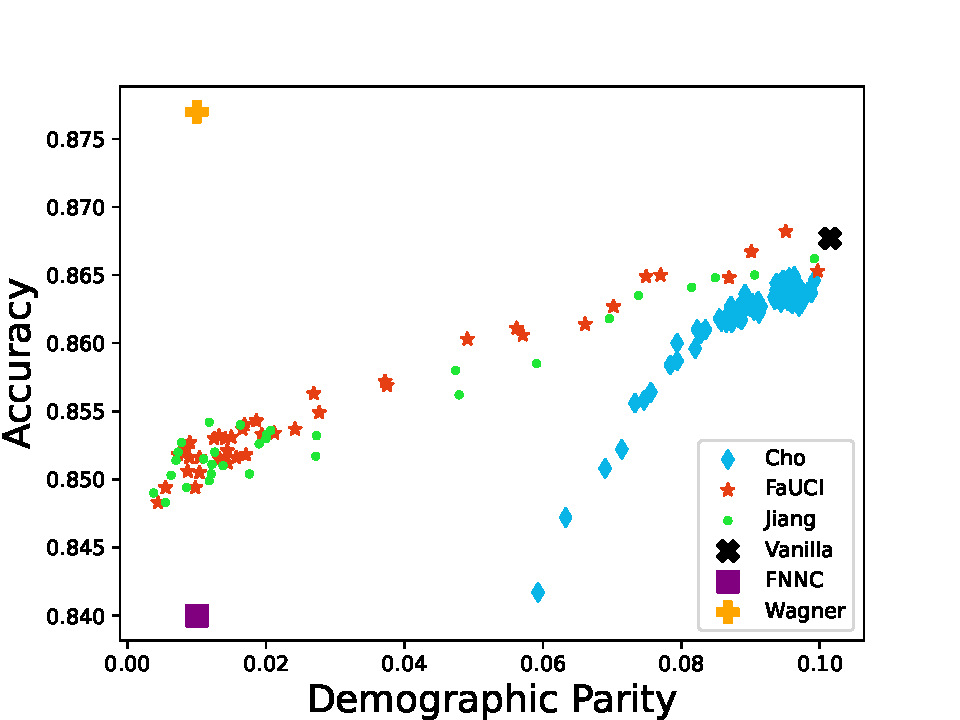
\includegraphics[width=\columnwidth]{figures/fauci/accuracy/demographic_parity_sex}
        \caption{Sensitive attribute: sex}
        \label{fig:dp-sex}
    \end{subfigure}
    %
    \begin{subfigure}[]{\onethirdsize}
        \centering
        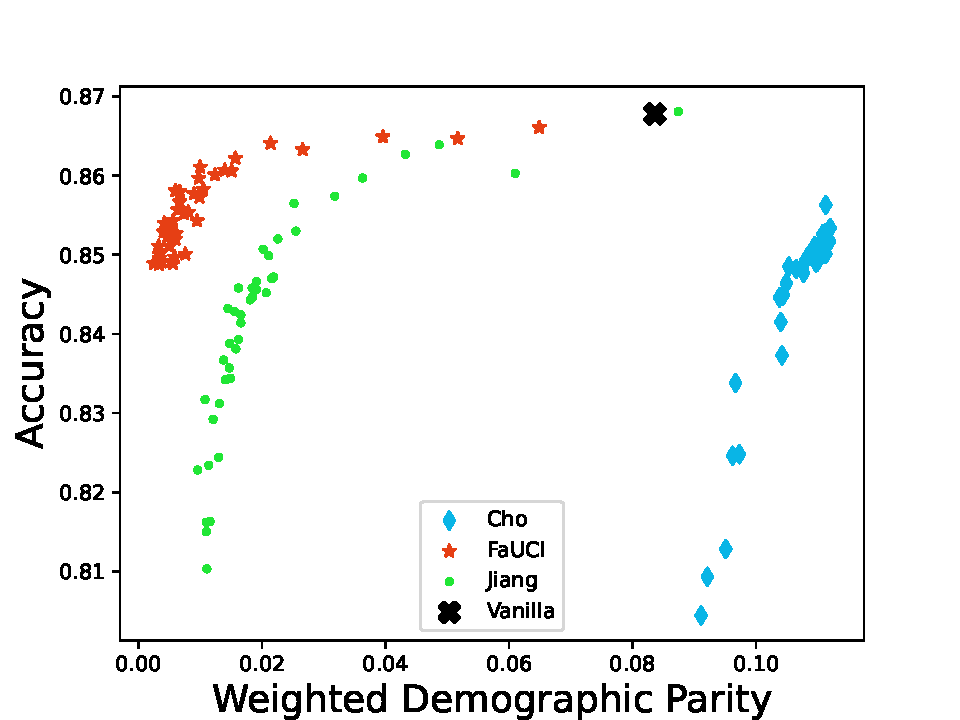
\includegraphics[width=\columnwidth]{figures/fauci/accuracy/demographic_parity_ethnicity}
        \caption{Sensitive attribute: ethnicity}
        \label{fig:dp-ethnicity}
    \end{subfigure}
    %
    \begin{subfigure}[]{\onethirdsize}
        \centering
        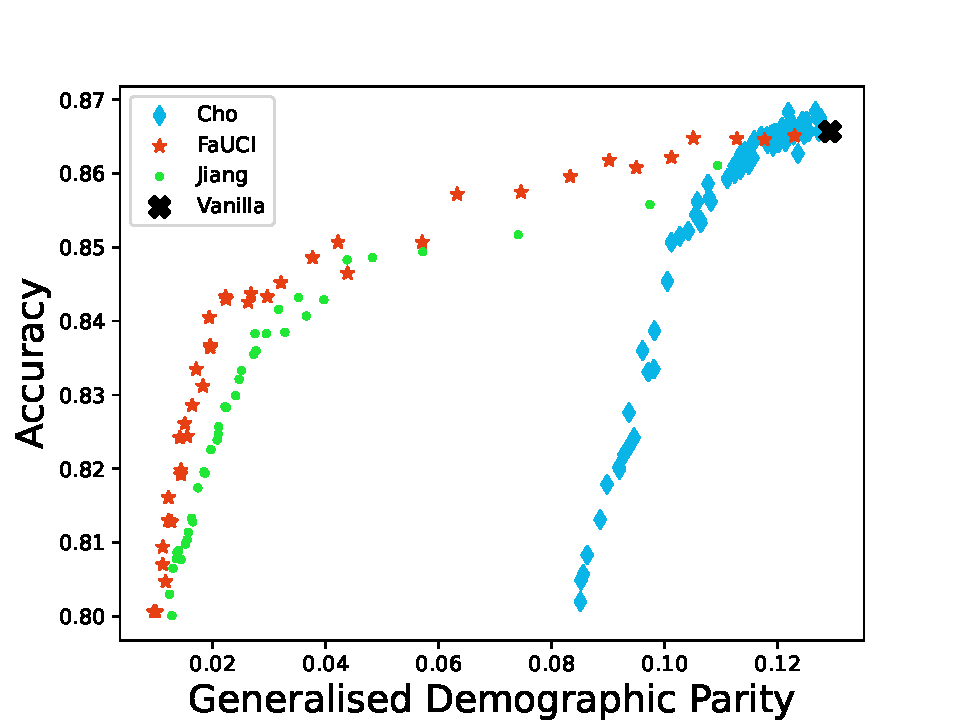
\includegraphics[width=\columnwidth]{figures/fauci/accuracy/demographic_parity_age}
        \caption{Sensitive attribute: age}
        \label{fig:dp-age}
    \end{subfigure}
    \label{fig:dp}
% \end{figure*}
% %
% \begin{figure*}[ht!]
%     \centering
%     \caption{%
%         Experiments applying DI constraints across different sensitive attributes. Legend as in \Cref{fig:dp}.
%         %
% %        Each dot is the average of 5 runs (5-folds cross-validation).
% %        %
% %        Red stars represent \fauci{}, the black cross the vanilla neural network (i.e., the NN without fairness constraints) and when possible, FNNC is represented as a purple square and Wagner's method as an orange cross.
%     }

    \begin{subfigure}[]{\onethirdsize}
        \centering
        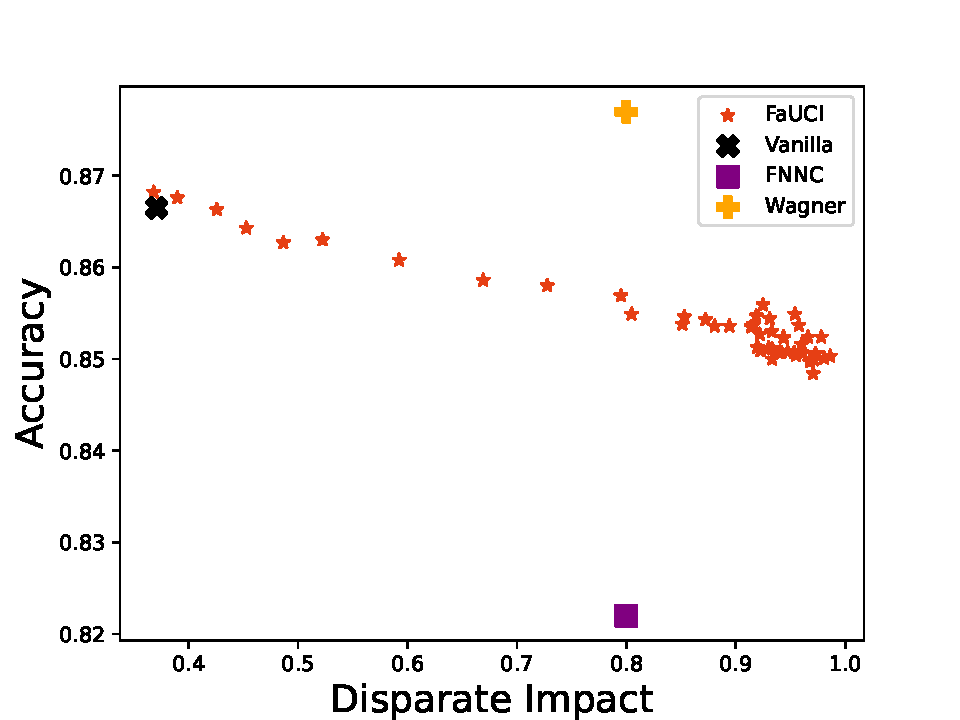
\includegraphics[width=\columnwidth]{figures/fauci/accuracy/disparate_impact_sex}
        \caption{Sensitive attribute: sex}
        \label{fig:di-sex}
    \end{subfigure}
    %
    \begin{subfigure}[]{\onethirdsize}
        \centering
        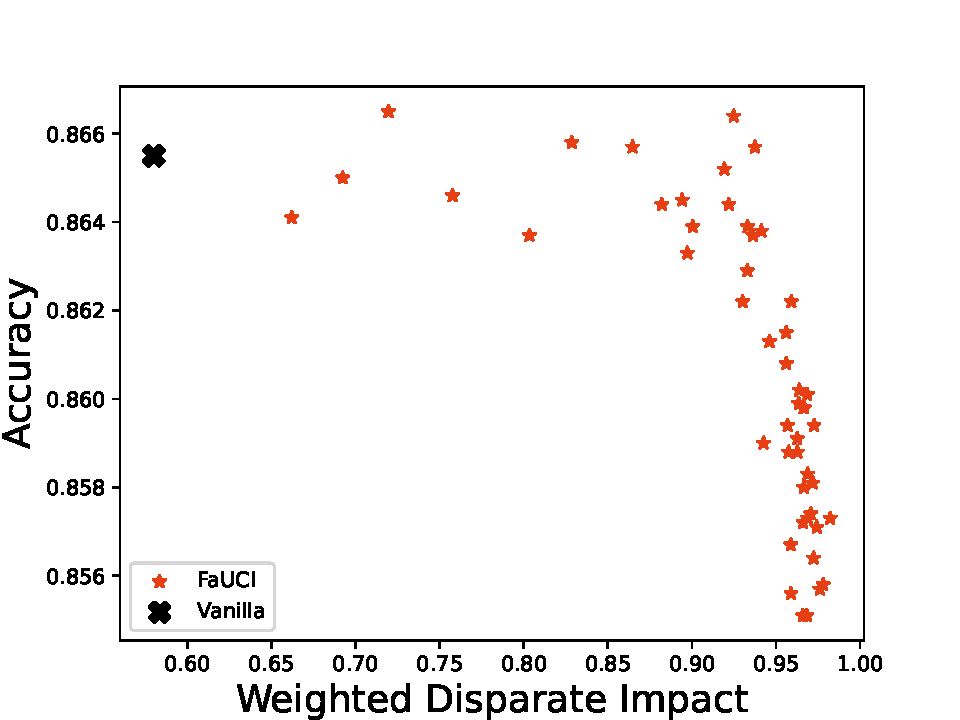
\includegraphics[width=\columnwidth]{figures/fauci/accuracy/disparate_impact_ethnicity}
        \caption{Sensitive attribute: ethnicity}
        \label{fig:di-ethnicity}
    \end{subfigure}
    %
    \begin{subfigure}[]{\onethirdsize}
        \centering
        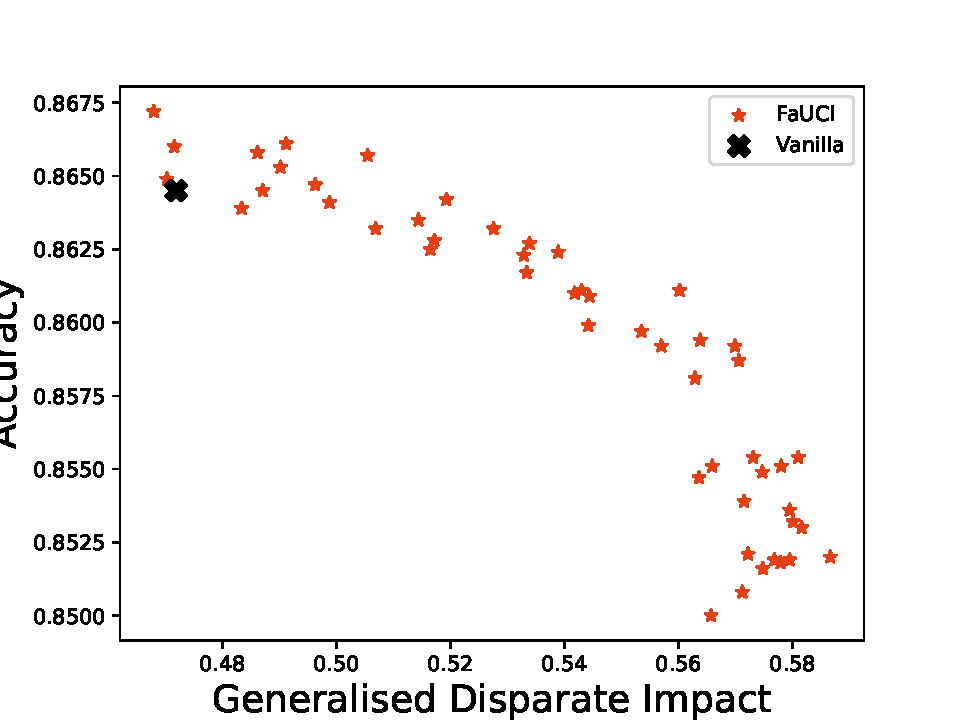
\includegraphics[width=\columnwidth]{figures/fauci/accuracy/disparate_impact_age}
        \caption{Sensitive attribute: age}
        \label{fig:di-age}
    \end{subfigure}
    \label{fig:di}
% \end{figure*}
% %
% \begin{figure*}[ht!]
%     \caption{%
%     	Experiments applying EO constraints across different sensitive attributes. Legend as in \Cref{fig:dp}.
%         %fairness methods results with different sensitive attributes.
%         %
% %        Each dot is the average of 5 runs (5-folds cross-validation).
% %        %
% %        Red stars represent our method, blue diamonds Cho's method, the black cross the vanilla neural network (i.e., the NN without fairness constraints) and when possible, FNNC is represented as a purple square.
%     }

    \begin{subfigure}[]{\onethirdsize}
        \centering
        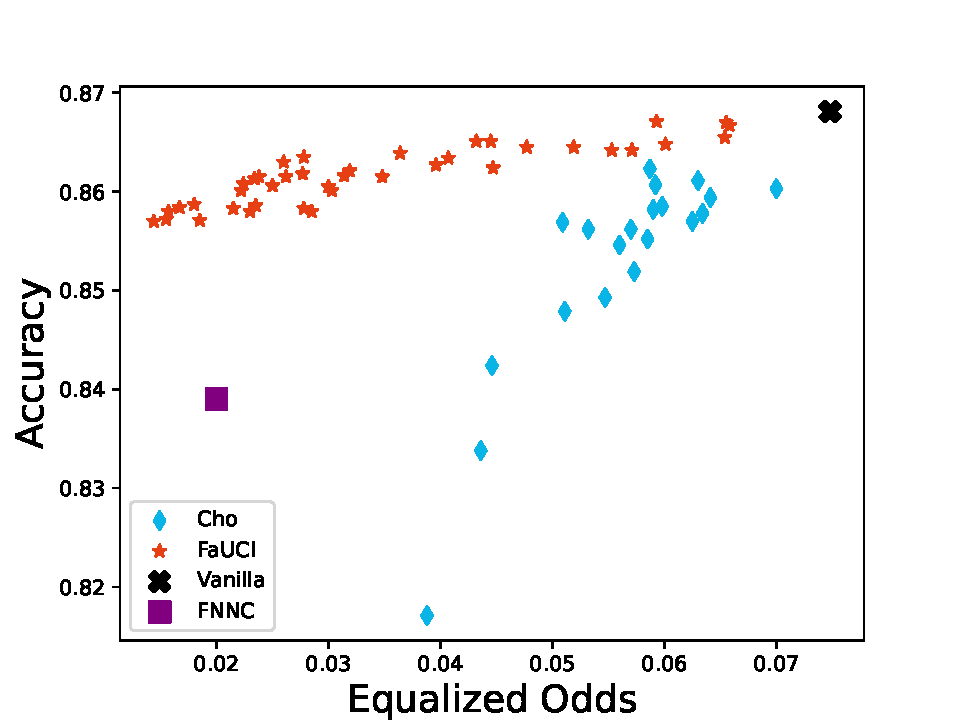
\includegraphics[width=\columnwidth]{figures/fauci/accuracy/equalized_odds_sex}
        \caption{Sensitive attribute: sex}
        \label{fig:eo-sex}
    \end{subfigure}
    %
    \begin{subfigure}[]{\onethirdsize}
        \centering
        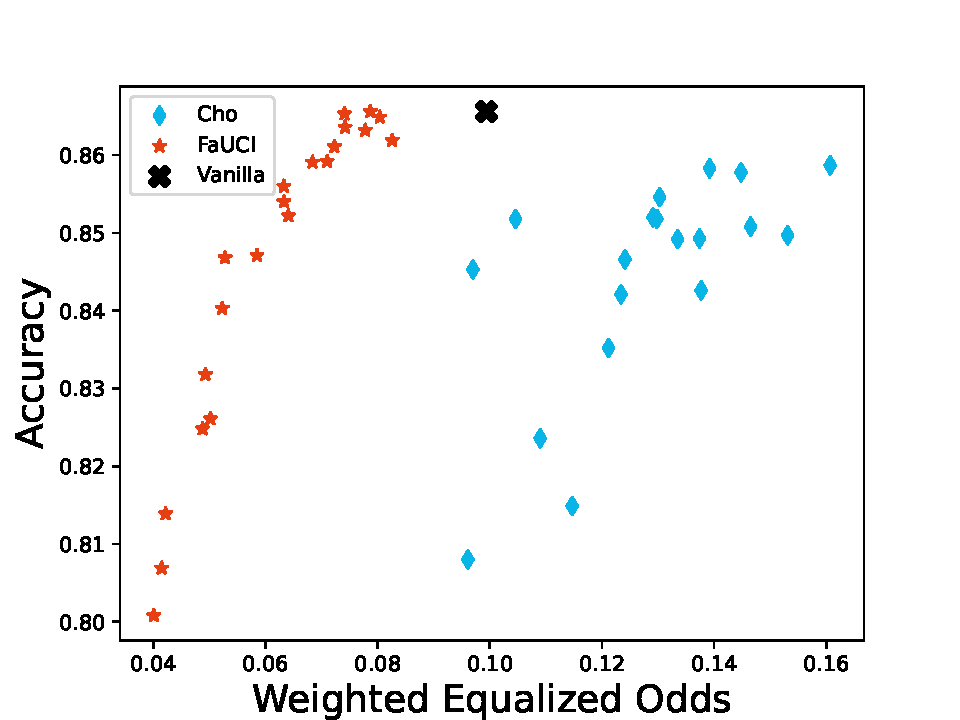
\includegraphics[width=\columnwidth]{figures/fauci/accuracy/equalized_odds_ethnicity}
        \caption{Sensitive attribute: ethnicity}
        \label{fig:eo-ethnicity}
    \end{subfigure}
    %
    \begin{subfigure}[]{\onethirdsize}
        \centering
        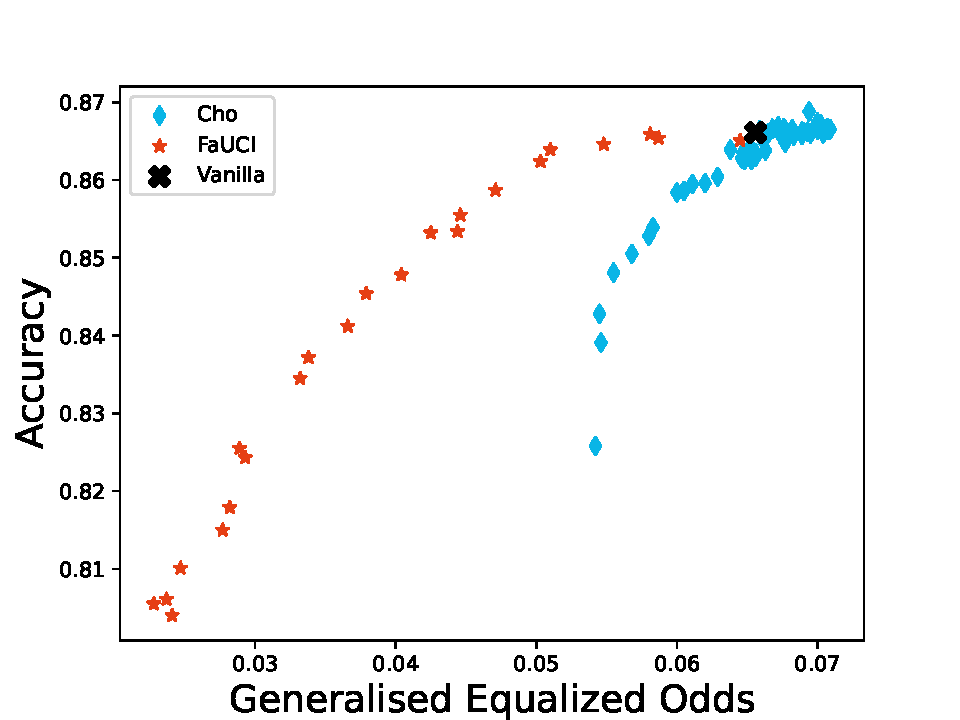
\includegraphics[width=\columnwidth]{figures/fauci/accuracy/equalized_odds_age}
        \caption{Sensitive attribute: age}
        \label{fig:eo-age}
    \end{subfigure}
    \label{fig:eo}
\end{figure}